\documentclass[11pt,letterpaper]{article}
\IfFileExists{spanish.ldf}{\usepackage[spanish,es-tabla,es-nodecimaldot]{babel}}{\usepackage{babel}}
\usepackage[utf8]{inputenc}
\usepackage[T1]{fontenc}
\usepackage{lmodern,microtype}
\usepackage[margin=1.8cm,top=1.9cm]{geometry}
\usepackage{amsmath,amssymb}
\usepackage{graphicx,xcolor,booktabs,tabularx,array,enumitem}
\usepackage{titlesec,fancyhdr,float}
\usepackage[hidelinks]{hyperref}
\usepackage{url}
\usepackage{listings}
\lstset{language=Python,basicstyle=\ttfamily\footnotesize,keywordstyle=\color{tecnmblue}\bfseries,commentstyle=\color{gray},stringstyle=\color{accentcolor},frame=single,rulecolor=\color{softblue},backgroundcolor=\color{softblue!40},columns=fullflexible,keepspaces=true,showstringspaces=false,literate={á}{{\'a}}1{é}{{\'e}}1{í}{{\'i}}1{ó}{{\'o}}1{ú}{{\'u}}1{ñ}{{\~n}}1}

\definecolor{tecnmblue}{RGB}{27,57,106}
\definecolor{accentcolor}{RGB}{229,103,31}
\definecolor{softblue}{RGB}{227,234,246}
\definecolor{softorange}{RGB}{252,236,226}

\titleformat{\section}{\large\bfseries\color{tecnmblue}}{\thesection.}{0.6em}{}
\titleformat{\subsection}{\normalsize\bfseries\color{tecnmblue}}{\thesubsection}{0.6em}{}
\titlespacing*{\section}{0pt}{1.1em}{0.5em}
\setlist{itemsep=2pt,topsep=3pt}
\setlength{\parindent}{0pt}\setlength{\parskip}{4pt}
\renewcommand{\arraystretch}{1.25}
\newcolumntype{Y}{>{\raggedright\arraybackslash}X}
\graphicspath{{img/}}

\pagestyle{fancy}\fancyhf{}
\lhead{\small\color{tecnmblue}Cálculo Vectorial Aplicado · ACF-0904}
\rhead{\small\color{tecnmblue}Proyecto Final U5 · Ejemplo guiado (código DEMO)}
\cfoot{\small\thepage}
\renewcommand{\headrulewidth}{0.4pt}

\newcommand{\paso}[1]{\par\smallskip{\color{accentcolor}\textbf{#1}}\par}
\newcommand{\aviso}[1]{\par\smallskip\colorbox{softorange}{\parbox{\dimexpr\linewidth-2\fboxsep}{\small #1}}\par\smallskip}
\newcommand{\resultado}[1]{\par\colorbox{softblue}{\parbox{\dimexpr\linewidth-2\fboxsep}{#1}}\par}

\begin{document}

\begin{center}
{\LARGE\bfseries\color{tecnmblue} Ejemplo guiado}\\[3pt]
{\large Proyecto Final: ruta de mínima energía para un dron de reparto}\\[3pt]
{\normalsize Resuelto paso a paso con los datos de práctica (código \texttt{DEMO})}
\end{center}

\aviso{\textbf{Cómo usar este ejemplo.} Aquí se resuelve el proyecto completo con los datos del código \texttt{DEMO}. \textbf{Sus datos son distintos}: copien el método, no los números. Consola: \url{https://thuerta2398.github.io/calculo-vectorial-u5-dron-sistemas/}}

\section{Paso 1 · Abrir la consola y leer la ficha técnica}
\begin{enumerate}
\item Abran la consola en la computadora o el celular. Al entrar ya carga \texttt{DEMO}; para su misión, escriban su código (\texttt{DRN-XXXX}) y pulsen \emph{Cargar misión}.
\item Copien la \textbf{ficha técnica} en su reporte. Con \texttt{DEMO} queda así:
\end{enumerate}

\begin{center}\small
\begin{tabularx}{0.95\linewidth}{@{}l Y@{}}
\toprule
Origen y destino & \(A=(0,0)\), \(B=(6,0)\) km \quad (\(L=6\), \(R=3\)) \\
Viento & \(\vec F=\langle -1+0.3\,x+0.15\,y^2,\;\; 7.5+0.05\,y^2-2.5\,x\rangle\) N \quad (\(u=1,\ b=0.3,\ a=0.15,\ d=7.5,\ e=0.05,\ c=2.5\)) \\
Ruta 2 & \(y=0.15\,x(6-x)\) \quad (\(k=0.15\)); vértice \(V=(3,\;1.35)\) \\
Ruta 3 & semicircunferencia superior de centro \((3,0)\) y radio \(3\) km \\
Energía & \(\varepsilon=12\) kJ/km; batería \(E_{\text{bat}}=90\) kJ; máximo por vuelo \(0.8(90)=72\) kJ \\ \bottomrule
\end{tabularx}
\end{center}

\begin{figure}[H]\centering
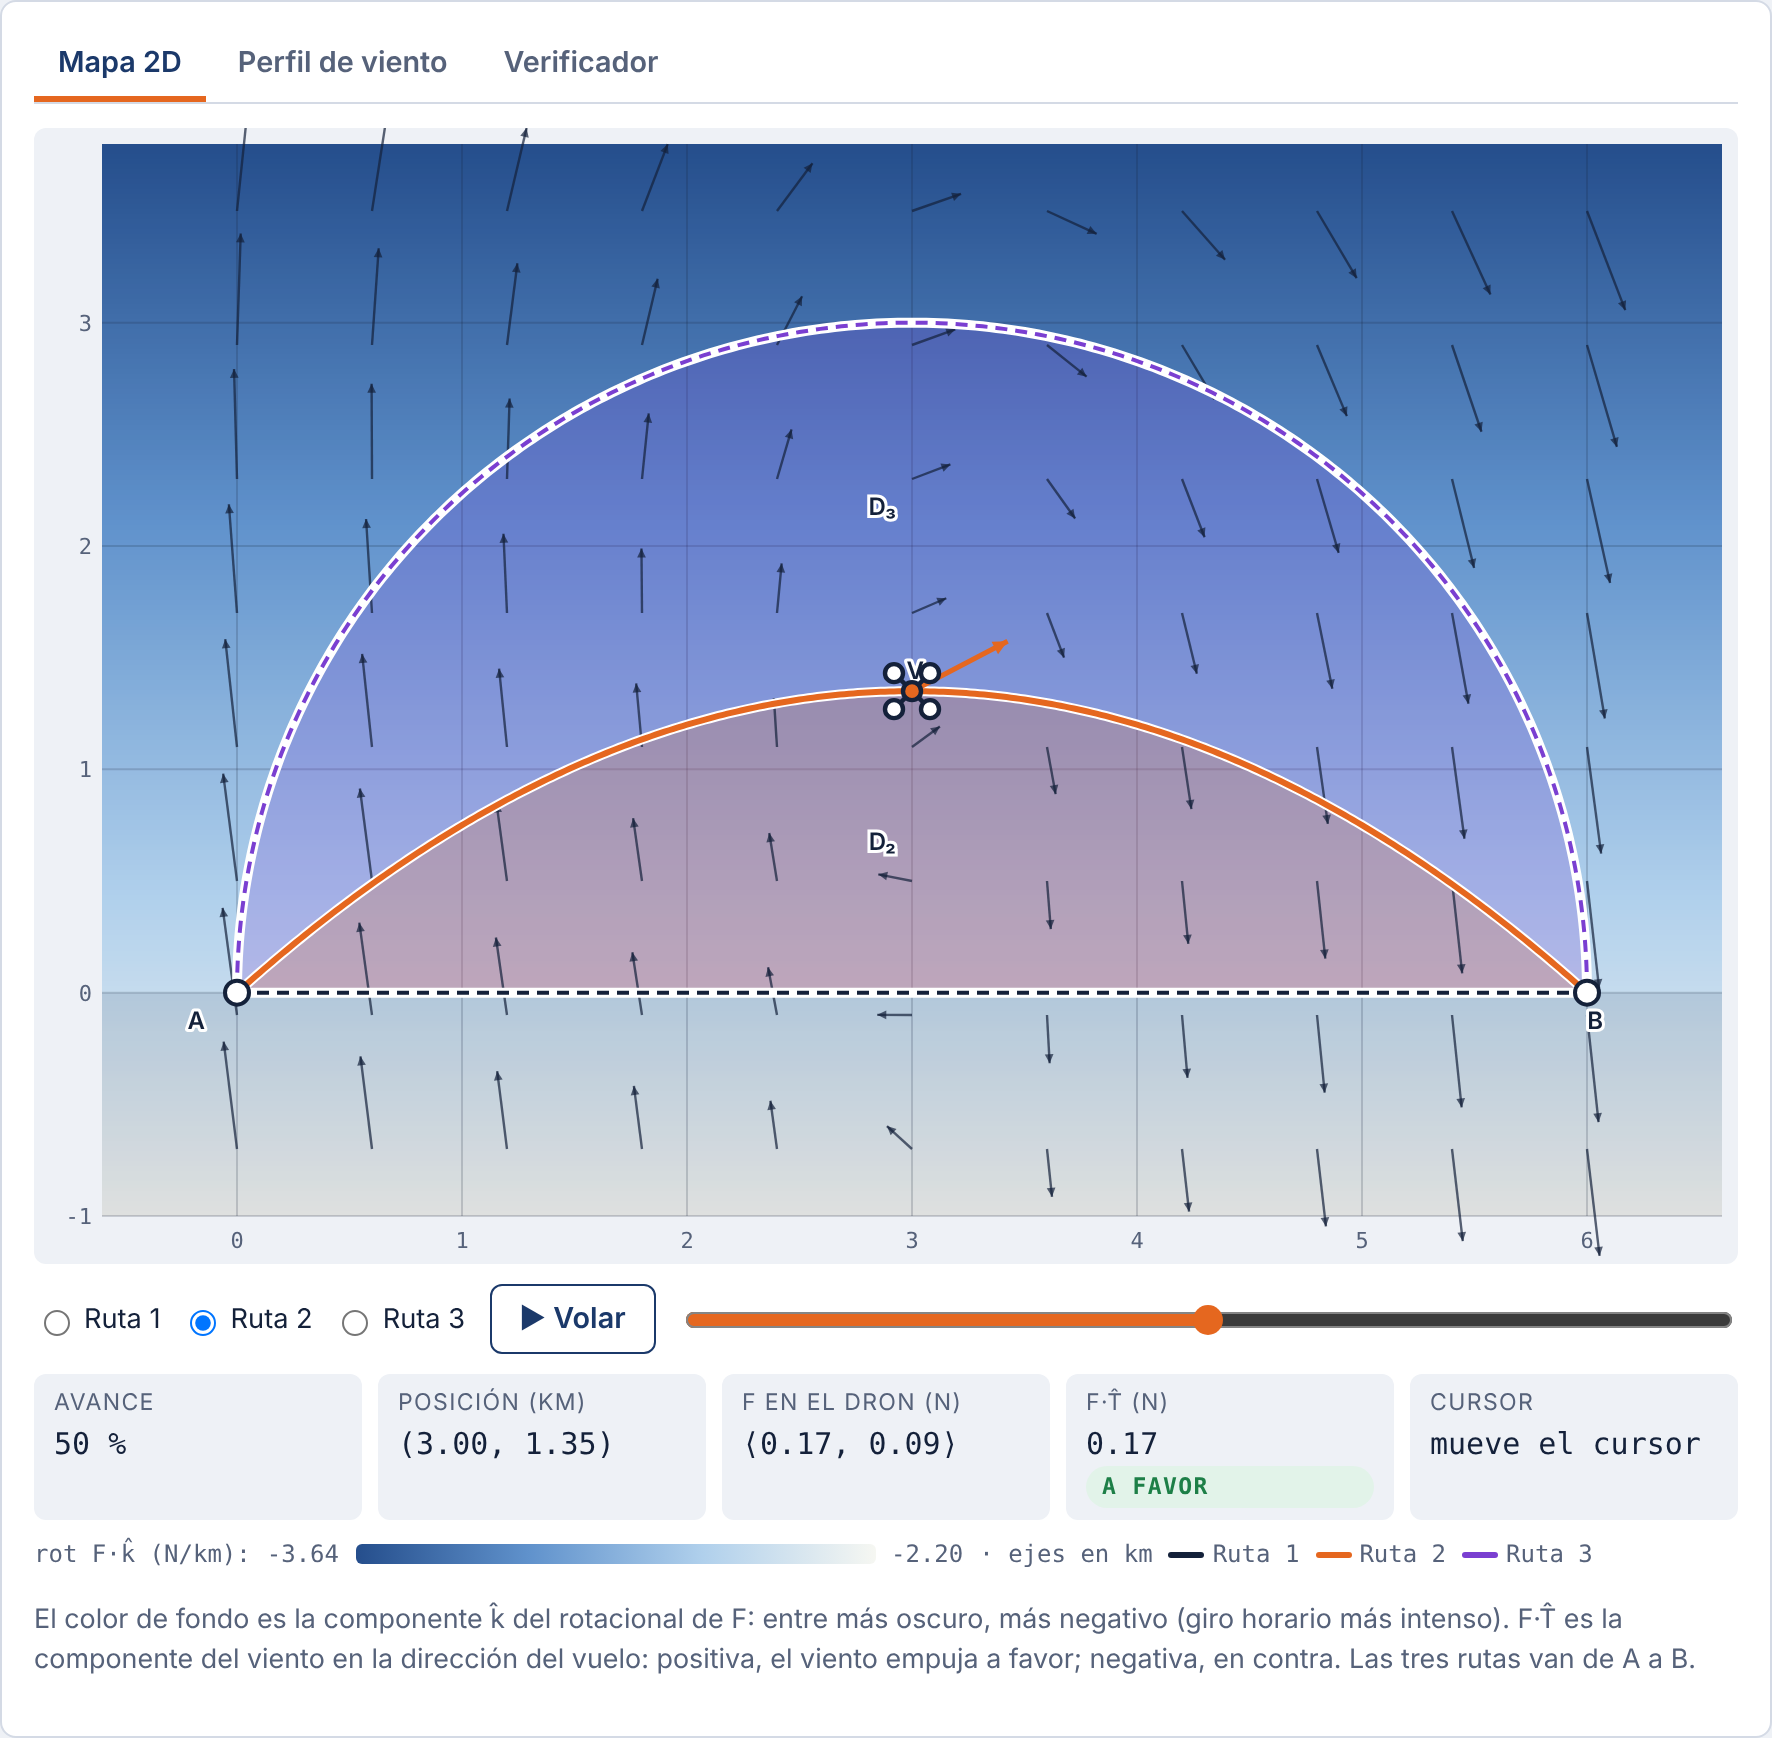
\includegraphics[height=0.40\textheight,keepaspectratio]{c1_mapa.png}
\caption{Mapa 2D con \texttt{DEMO}: rotacional de \(\vec F\) (fondo), campo \(\vec F\) (flechas), rutas 1 (negra), 2 (naranja) y 3 (morada), regiones \(D_2\) y \(D_3\), y el dron sobre la Ruta 2 en el vértice \(V\).}
\end{figure}

\paso{Qué observar antes de calcular}
\begin{itemize}
\item Sobre la costa (\(y=0\)) la componente \(P=-1+0.3x\) es negativa al inicio: la brisa frena al dron cerca de \(A\).
\item Tierra adentro el término \(0.15\,y^2\) hace que el viento empuje hacia el este: las rutas que se alejan de la costa reciben más ayuda, pero son más largas.
\item En el \emph{Perfil de viento}, la curva de la Ruta 3 queda casi siempre arriba de las demás. El área bajo cada curva es \(W_i\): anticipa el orden \(W_1<W_2<W_3\).
\end{itemize}

\section{Paso 2 · Solución por rol}

\subsection*{Ingeniero de Logística: trabajo sobre las rutas 1 y 2}
\paso{a) Ruta 1: \(y=0\), \(dy=0\), \(x\) de 0 a 6}
\[W_1=\int_0^6 P(x,0)\,dx=\int_0^6(-1+0.3x)\,dx=\Big[-x+0.15x^2\Big]_0^6=-6+5.4=\mathbf{-0.60\ kJ}.\]
\paso{b) Ruta 2: parametrizar}
\(x=t,\quad y=0.15t(6-t)=0.9t-0.15t^2,\quad dx=dt,\quad dy=(0.9-0.3t)\,dt,\quad t\in[0,6].\)
\paso{c) Término \(P\,dx\)}
\begin{align*}
\int_0^6\big(-1+0.3t\big)dt+0.15\int_0^6 y^2\,dt&=-0.6+0.15(0.15)^2\int_0^6 t^2(6-t)^2dt\\
&=-0.6+0.003375\cdot\frac{6^5}{30}=-0.6+0.8748=0.2748 .
\end{align*}
\paso{d) Término \(Q\,dy\)}
\[\int_C 7.5\,dy=7.5\,[y]_{0}^{0}=0,\qquad \int_C 0.05\,y^2\,dy=0.05\Big[\frac{y^3}{3}\Big]_{0}^{0}=0,\]
porque la ruta empieza y termina en \(y=0\). Solo queda el término con \(x\):
\[\int_0^6-2.5\,t\,(0.9-0.3t)\,dt=-2.5\Big[0.45t^2-0.1t^3\Big]_0^6=-2.5(16.2-21.6)=13.5 .\]
\resultado{\(W_2=0.2748+13.5=\mathbf{13.7748\ kJ}\). En la recta el viento casi no hace trabajo (\(W_1=-0.60\) kJ, ligeramente en contra); sobre la parábola el viento \textbf{ayuda} al dron.}

\subsection*{Ingeniero de Dinámica: divergencia y rotacional}
\paso{a) Derivadas parciales}
\(\dfrac{\partial P}{\partial x}=0.3,\quad \dfrac{\partial P}{\partial y}=0.3\,y,\quad \dfrac{\partial Q}{\partial x}=-2.5,\quad \dfrac{\partial Q}{\partial y}=0.1\,y.\)
\paso{b) Evaluar en \(V=(3,\,1.35)\)}
\begin{align*}
\operatorname{div}\vec F&=0.3+0.1y &&\Rightarrow\; 0.3+0.1(1.35)=\mathbf{0.435\ N/km}\\
(\operatorname{rot}\vec F)\cdot\hat k&=-2.5-0.3y &&\Rightarrow\; -2.5-0.3(1.35)=\mathbf{-2.905\ N/km}
\end{align*}
\paso{c) Interpretar}
\(\operatorname{div}>0\): en \(V\) el aire se expande (\textbf{fuente}). \(\operatorname{rot}<0\) en toda la zona \(y\ge 0\): el aire tiende a girar en sentido \textbf{horario}. Como el rotacional no es cero, \(\vec F\) \textbf{no es conservativo} y el trabajo depende de la ruta, aunque todas unan \(A\) con \(B\).

\subsection*{Analista de Zona: integrales dobles del rotacional}
\paso{a) \(D_2\) en rectangulares}
Con \(y_s(x)=0.15x(6-x)\): \(\displaystyle\int_0^{y_s}(-2.5-0.3y)\,dy=-2.5\,y_s-0.15\,y_s^2\), y
\[\int_0^6 y_s\,dx=0.15(36)=5.4,\qquad \int_0^6 y_s^2\,dx=0.0225(259.2)=5.832 .\]
\[I_2=-2.5(5.4)-0.15(5.832)=-13.5-0.8748=\mathbf{-14.3748\ kJ}.\]
\paso{b) \(D_3\) en polares centradas en \((3,0)\)}
Con \(x=3+r\cos\theta\), \(y=r\sin\theta\), \(dA=r\,dr\,d\theta\):
\[I_3=\int_0^{\pi}\!\!\int_0^{3}\big(-2.5-0.3\,r\sin\theta\big)\,r\,dr\,d\theta
=-2.5\cdot\frac{\pi(3)^2}{2}-0.3\Big[-\cos\theta\Big]_0^{\pi}\Big[\frac{r^3}{3}\Big]_0^{3}
=-11.25\pi-5.4=\mathbf{-40.7429\ kJ}.\]

\subsection*{Gerente de Calidad: \(W_3\) directo y teorema de Green}
\paso{a) Parametrizar la semicircunferencia (\(\theta\) de \(\pi\) a \(0\))}
\(x=3+3\cos\theta,\ y=3\sin\theta,\ dx=-3\sin\theta\,d\theta,\ dy=3\cos\theta\,d\theta\). Al sustituir:
\[P=-0.1+0.9\cos\theta+1.35\sin^2\theta,\qquad Q=0.45\sin^2\theta-7.5\cos\theta .\]
\paso{b) Integrar}
\[P\,dx+Q\,dy=\big(0.3\sin\theta-2.7\sin\theta\cos\theta-4.05\sin^3\theta+1.35\sin^2\theta\cos\theta-22.5\cos^2\theta\big)d\theta .\]
\[\int_0^{\pi}(\ldots)\,d\theta=0.6-0-4.05\cdot\tfrac43+0-22.5\cdot\tfrac{\pi}{2}=0.6-5.4-11.25\pi=-40.1429 .\]
\resultado{Como \(\theta\) va de \(\pi\) a \(0\), \(W_3=-\int_0^{\pi}(\ldots)\,d\theta=\mathbf{40.1429\ kJ}\).}
\paso{c) Comprobar Green (contorno antihorario: \(A\to B\) por la recta y regreso por la ruta curva)}
\[W_1-W_2=-0.60-13.7748=-14.3748=I_2\ \checkmark\qquad W_1-W_3=-0.60-40.1429=-40.7429=I_3\ \checkmark\]
\resultado{Green explica la diferencia: como \(\operatorname{rot}\vec F<0\) en la región entre las rutas, \(W_1-W_i<0\), es decir, \(W_i>W_1\). Entre más área de rotacional negativo encierra una ruta, más la ayuda el viento.}

\section{Paso 3 · Python: longitud, energía y decisión}
Completen la plantilla. Estos son los fragmentos clave con los datos \texttt{DEMO}:
\begin{lstlisting}
def trabajo(i):
    r, dr, t0, t1 = RUTAS[i]
    return quad(lambda t: F(*r(t)) @ dr(t), t0, t1)[0]

def longitud(i):
    r, dr, t0, t1 = RUTAS[i]
    return abs(quad(lambda t: np.linalg.norm(dr(t)), t0, t1)[0])

I3 = dblquad(lambda th, r: rot(R + r*np.cos(th), r*np.sin(th)) * r, 0, R, 0, math.pi)[0]
\end{lstlisting}
Salida del programa:
\begin{lstlisting}[language={}]
Ruta 1: W = -0.6000 kJ  l = 6.0000 km  E = 72.6000 kJ  (NO fact.)
Ruta 2: W = 13.7748 kJ  l = 6.7323 km  E = 67.0129 kJ  (fact.)
Ruta 3: W = 40.1429 kJ  l = 9.4248 km  E = 72.9544 kJ  (NO fact.)
Green (D2, D3): (True, True)
Ruta más económica: 2  E = 67.0129 kJ
\end{lstlisting}
\begin{figure}[H]\centering
\begin{minipage}{0.58\linewidth}\centering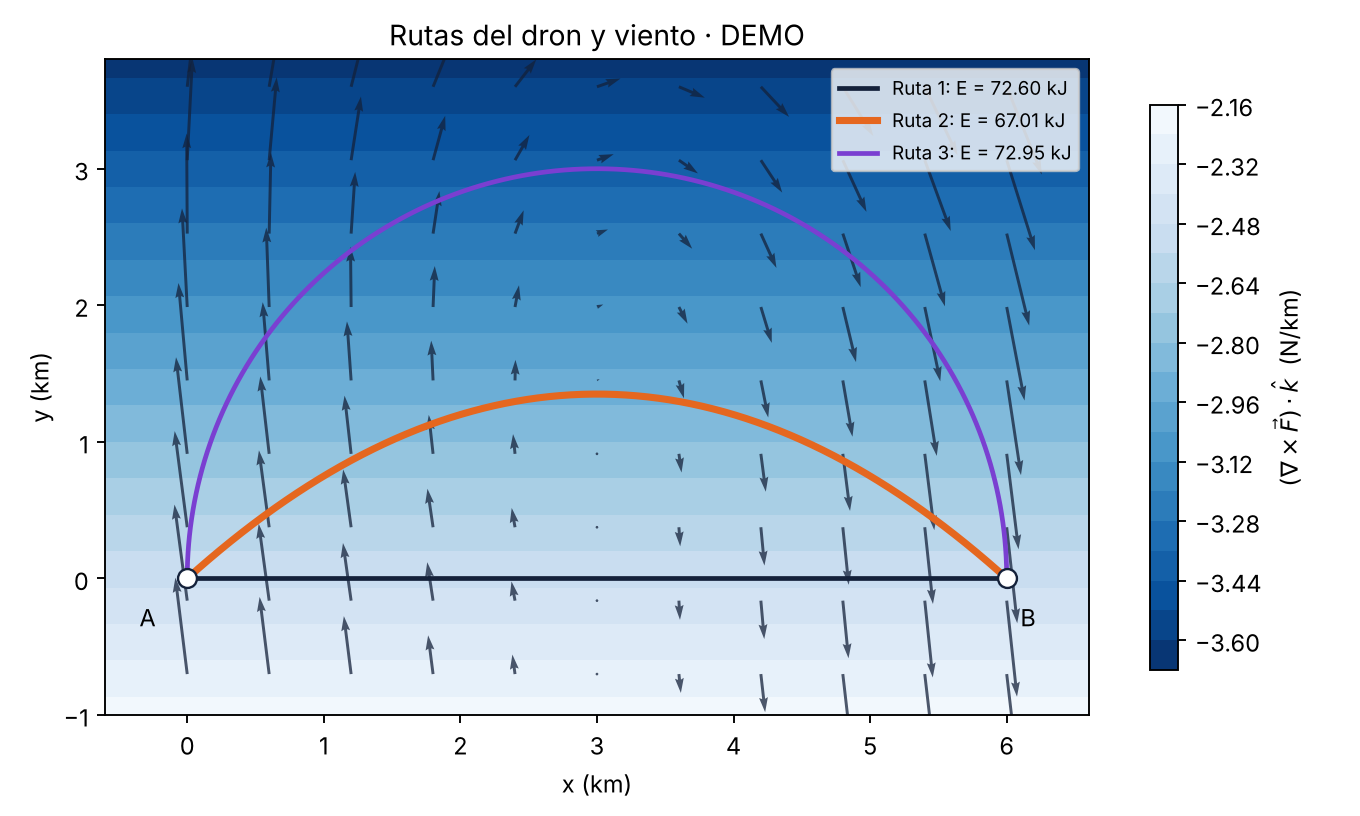
\includegraphics[width=\linewidth]{mapa_DEMO.png}\end{minipage}\hfill
\begin{minipage}{0.40\linewidth}\centering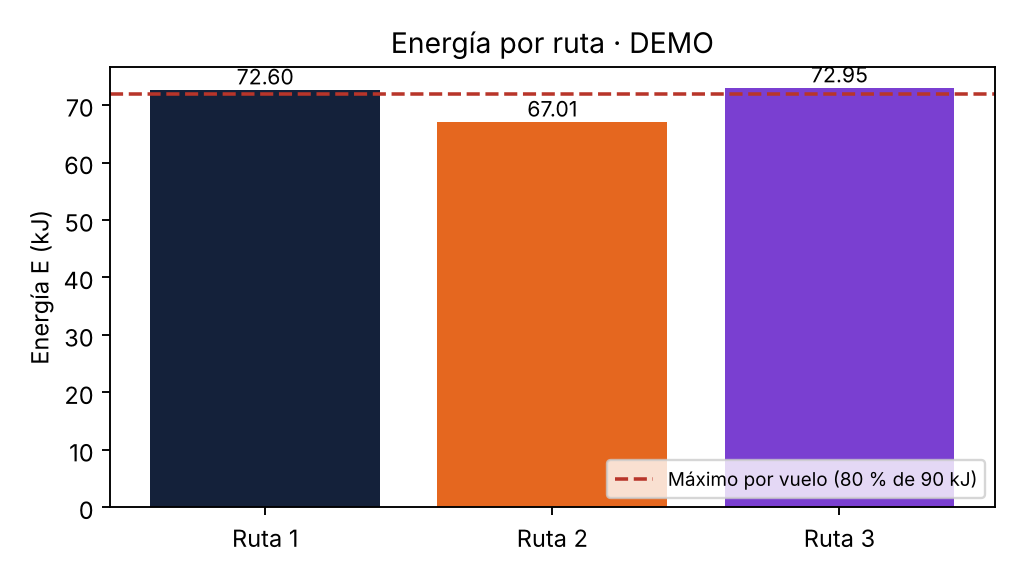
\includegraphics[width=\linewidth]{energia_DEMO.png}\end{minipage}
\caption{Figuras generadas con Python para \texttt{DEMO}: mapa del rotacional con el campo y las rutas (izquierda) y energía por ruta frente al máximo por vuelo de 72 kJ (derecha). La animación \texttt{vuelo\_DEMO.gif} muestra los tres drones volando a la vez.}
\end{figure}
\aviso{\textbf{La longitud de la parábola.} \(\ell_2=\int_0^6\sqrt{1+(0.9-0.3t)^2}\,dt\approx 6.7323\) km. Tiene forma cerrada con \(\operatorname{senh}^{-1}\), pero calcularla con \texttt{quad} es lo esperado. Las otras dos son directas: \(\ell_1=6\), \(\ell_3=3\pi\approx 9.4248\).}

\section{Paso 4 · Verificar en la consola}
Capturen cada resultado con \textbf{punto decimal}, sin unidades. Si usan coma, la consola lo indica y ese intento no cuenta:
\begin{center}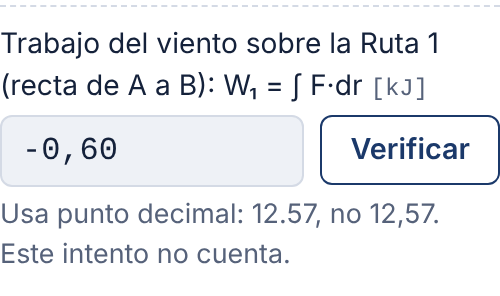
\includegraphics[width=0.28\linewidth]{c4_coma.png}\end{center}
Con los 9 resultados correctos aparece el folio. Con \texttt{DEMO} solo se muestra ``Práctica completa''; con su código aparece un folio del tipo \texttt{DRN-XXXX-1A2B3C4}, que va en la portada.
\begin{figure}[H]\centering
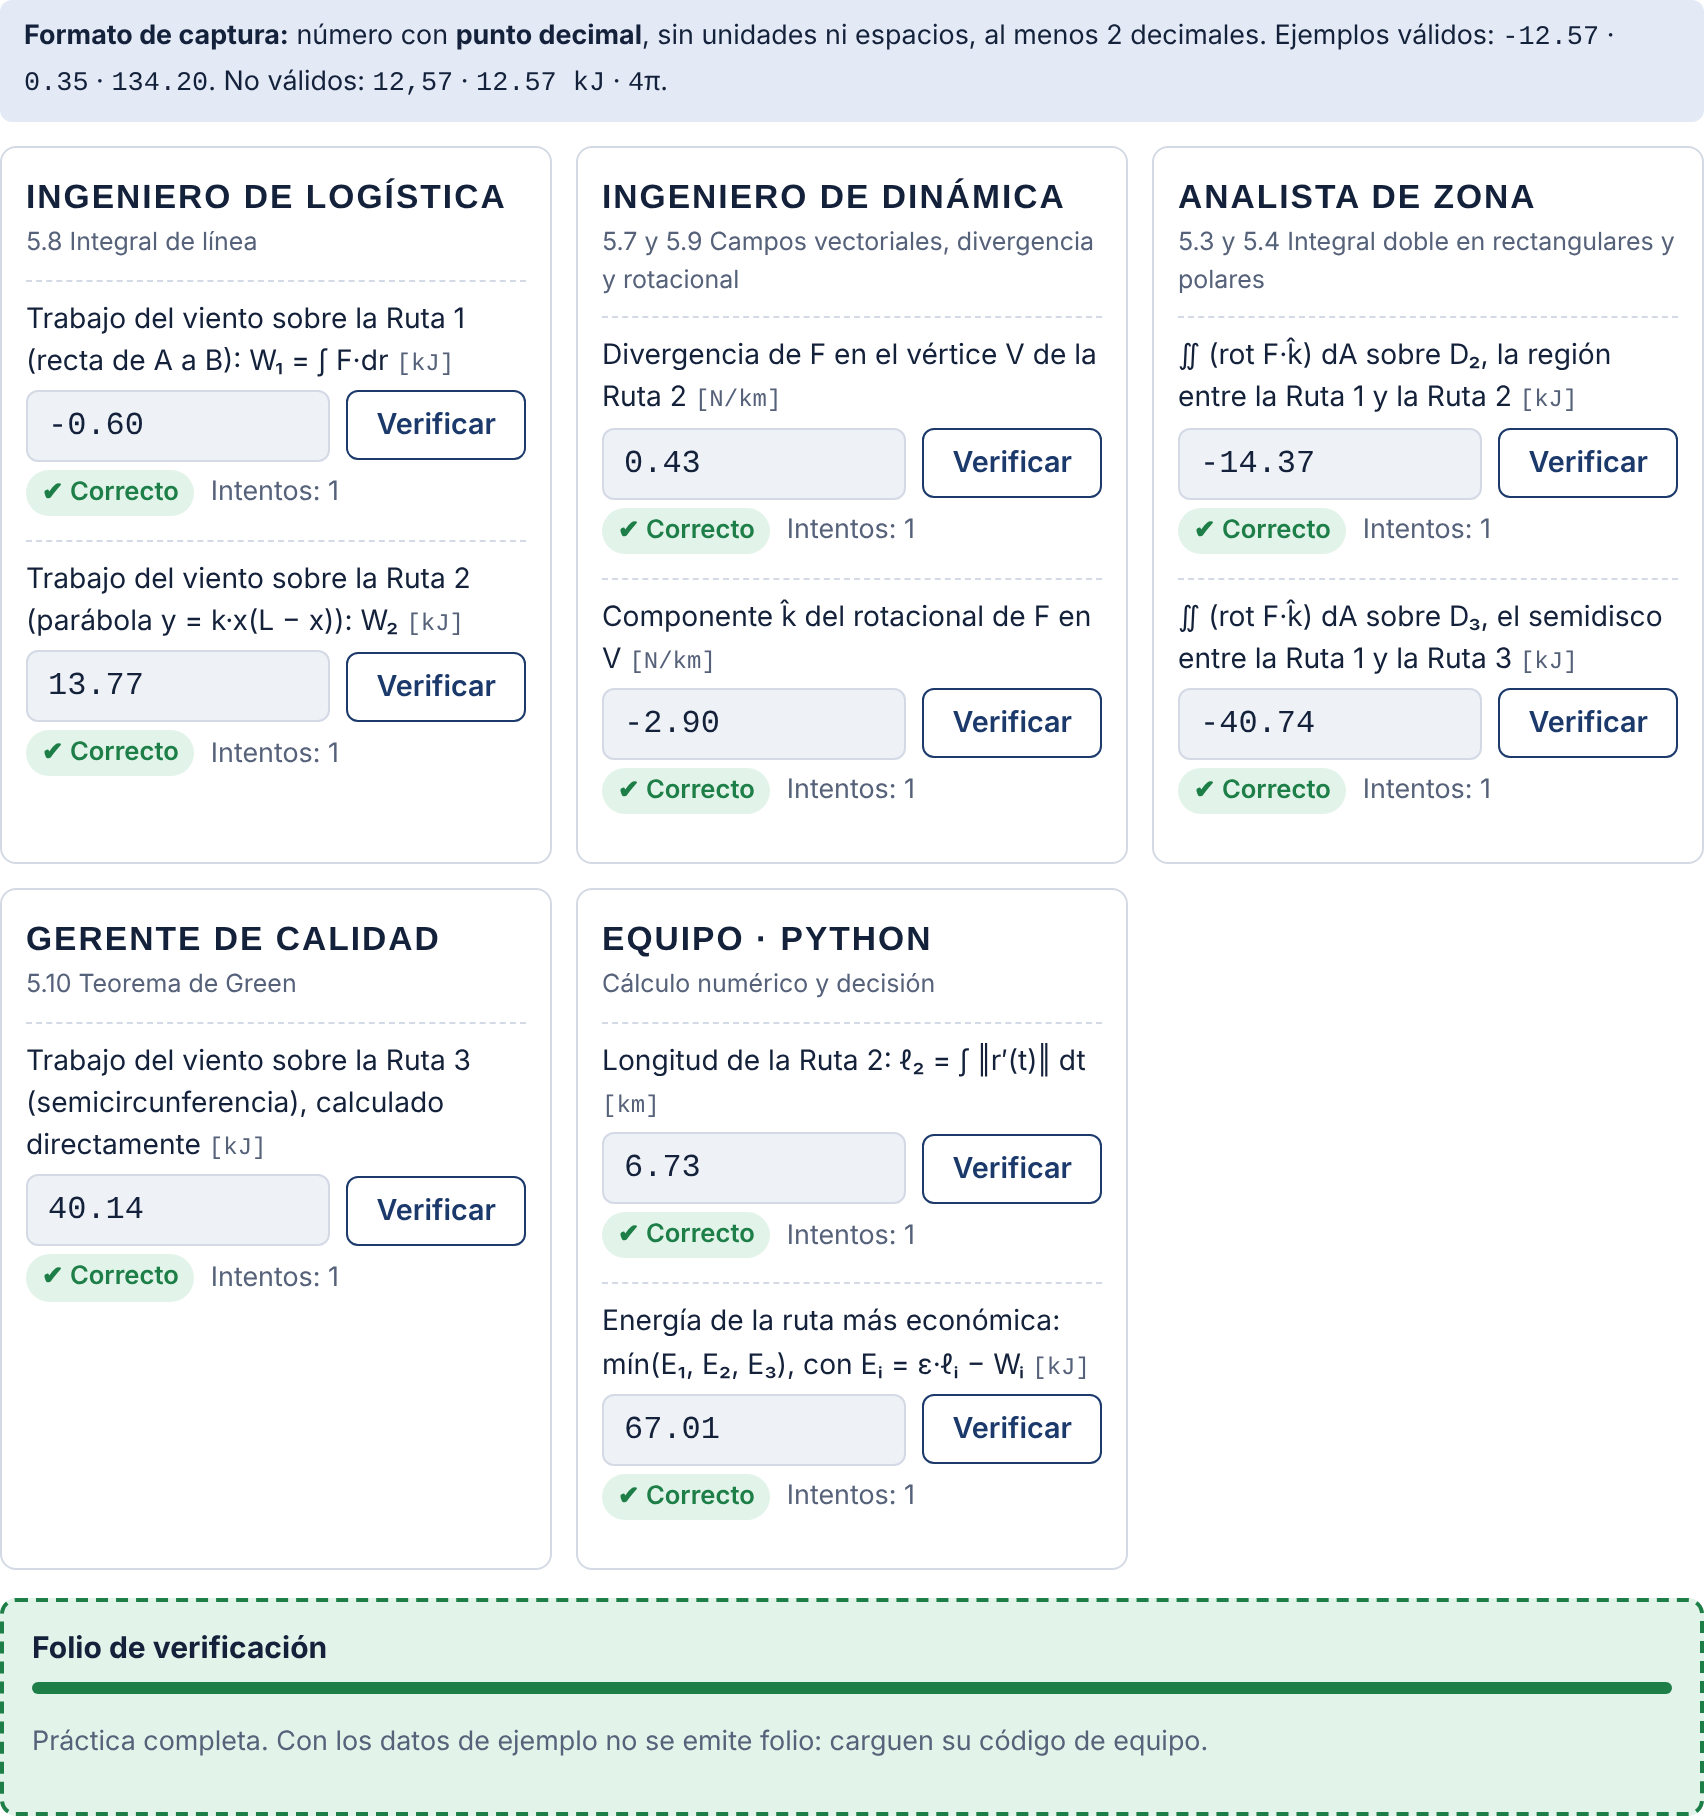
\includegraphics[width=0.62\linewidth]{c5_verificador.png}
\caption{Verificador con los 9 resultados de \texttt{DEMO} correctos.}
\end{figure}

\section{Paso 5 · Redactar el dictamen (ejemplo)}
\resultado{\small\textbf{Dictamen de ingeniería (código DEMO).}
\textbf{Energía y factibilidad:} las energías son \(E_1=72.60\), \(E_2=67.01\) y \(E_3=72.95\) kJ. Con la reserva del 20~\%, el máximo por vuelo es 72 kJ: solo la Ruta 2 es factible, con una reserva de \(1-67.01/90\approx 26~\%\).
\textbf{Efecto del viento:} en la recta el viento casi no trabaja (\(W_1=-0.60\) kJ); en la parábola aporta \(W_2=13.77\) kJ y en la semicircunferencia \(W_3=40.14\) kJ. La recta es la más corta, pero no aprovecha el viento; la semicircunferencia lo aprovecha más, pero es 57~\% más larga. La parábola equilibra ambos efectos.
\textbf{Rotacional y Green:} \(\operatorname{rot}\vec F=-2.905\) N/km en \(V\) y es negativo en toda la zona de vuelo, así que \(\vec F\) no es conservativo. Con Green, \(W_1-W_2=I_2=-14.37\) kJ y \(W_1-W_3=I_3=-40.74\) kJ: la ganancia de cada ruta curva es el rotacional acumulado en el área que encierra. En \(V\), \(\operatorname{div}\vec F=0.435>0\) (fuente).
\textbf{Decisión: ruta aprobada, Ruta 2 (parábola)}, con 26~\% de reserva de batería.}

Fíjense en que cada afirmación del dictamen \textbf{usa un número calculado} y termina en una consecuencia para la misión.

\clearpage
\section{Paso 6 · Armar la entrega}
\subsection*{Portada (ejemplo)}
\begin{center}\small
\begin{tabularx}{0.9\linewidth}{@{}l Y@{}}\toprule
Código de equipo & \texttt{DRN-XXXX} \\
Folio de verificación & \texttt{DRN-XXXX-1A2B3C4} (el que da su consola) \\
Integrantes y rol & Nombre 1: Logística · Nombre 2: Dinámica · Nombre 3: Análisis de Zona · Nombre 4: Calidad \\
Video & \url{https://drive.google.com/file/d/...} \\
Código & \url{https://github.com/usuario/proyecto-dron} o enlace de Colab \\ \bottomrule
\end{tabularx}\end{center}

\subsection*{El código}
\begin{itemize}
\item \textbf{GitHub (recomendado):} creen un repositorio público, suban \texttt{dron\_plantilla.py} completo, el GIF y las figuras. Que cada integrante haga \emph{commit} de su bloque: el historial muestra la participación.
\item \textbf{Google Colab:} abran \texttt{dron\_plantilla.ipynb} (\emph{Archivo \(\rightarrow\) Subir cuaderno}), complétenlo y compártanlo con \emph{Cualquier persona con el enlace · Lector}.
\item Antes de entregar, ejecuten todo desde cero (\emph{Entorno de ejecución \(\rightarrow\) Reiniciar y ejecutar todo}): debe correr sin errores.
\end{itemize}

\subsection*{El reporte en PDF (máximo 4 cuartillas, sin contar la portada)}
\begin{itemize}
\item \textbf{Word o Google Docs:} \emph{Insertar \(\rightarrow\) Ecuación}; al terminar, exporten a PDF.
\item \textbf{Procedimiento a mano:} es válido si se lee bien. Escaneen con la app de Google Drive o con Microsoft Lens e inserten las imágenes.
\item Para no pasarse de 4 cuartillas: una sección por rol (½ a ¾ de cuartilla cada una), el mapa y la gráfica de energía, y el dictamen al final.
\end{itemize}

\subsection*{El video (4:30 a 5:30 min, todos a cuadro, con rotación de roles)}
\begin{enumerate}
\item \textbf{Grabar:} videollamada en Zoom, Teams o Meet con las cuatro cámaras encendidas; compartan la animación y la consola en pantalla y graben la reunión.
\item \textbf{Guion sugerido}, alrededor de 1 min por persona: Logística explica Dinámica, Dinámica explica Análisis de Zona, Análisis de Zona explica Calidad y Calidad explica Logística. Cierren con el dictamen en 30 s.
\item \textbf{Subir y compartir en Drive:} \emph{Compartir \(\rightarrow\) Acceso general \(\rightarrow\) ``Cualquier persona con el enlace'' · Lector \(\rightarrow\) Copiar vínculo}.
\item \textbf{Probar:} abran el vínculo en una ventana de incógnito. Si pide iniciar sesión, el permiso está mal y el video valdría 0.
\end{enumerate}

\section{Errores frecuentes}
\begin{center}\small
\begin{tabularx}{\linewidth}{@{}>{\raggedright\arraybackslash}p{5.2cm} Y@{}}\toprule
\textbf{Error} & \textbf{Cómo evitarlo}\\\midrule
Recorrer la Ruta 3 de \(B\) a \(A\) & \(\theta\) va de \(\pi\) a \(0\). Si integran de \(0\) a \(\pi\), cambien el signo al final. \\
Olvidar \(dy\) en la Ruta 2 & \(dy=k(L-2t)\,dt\): sin él desaparece el término que más pesa. \\
Olvidar el factor \(r\) en polares & \(dA=r\,dr\,d\theta\), no \(dr\,d\theta\). \\
Signo en Green & El contorno antihorario es \(A\to B\) por la recta y regreso por la curva: \(W_1-W_i=\iint_{D_i}\operatorname{rot}\vec F\,dA\). \\
\texttt{dblquad} con argumentos al revés & \texttt{dblquad} integra \texttt{f(y, x)}: la variable interna va primero. \\
Calculadora en grados & Las integrales trigonométricas usan \textbf{radianes}. \\
Coma decimal o unidades en el verificador & \texttt{-14.37}, no \texttt{-14,37} ni \texttt{-14.37 kJ}. \\
Leer en el video & Ensayen una vez; usen la animación como apoyo visual, no un guion. \\ \bottomrule
\end{tabularx}\end{center}

\end{document}
